%---------------------------------------------------------------------------
% System Decomposition.
%
%---------------------------------------------------------------------------
\section{Decomposition}
\label{sec:arch_decomposition}

The high level system architecture is depicted in Figure~\ref{fig:arch_overall}. 

\begin{figure}[ht]
\centering
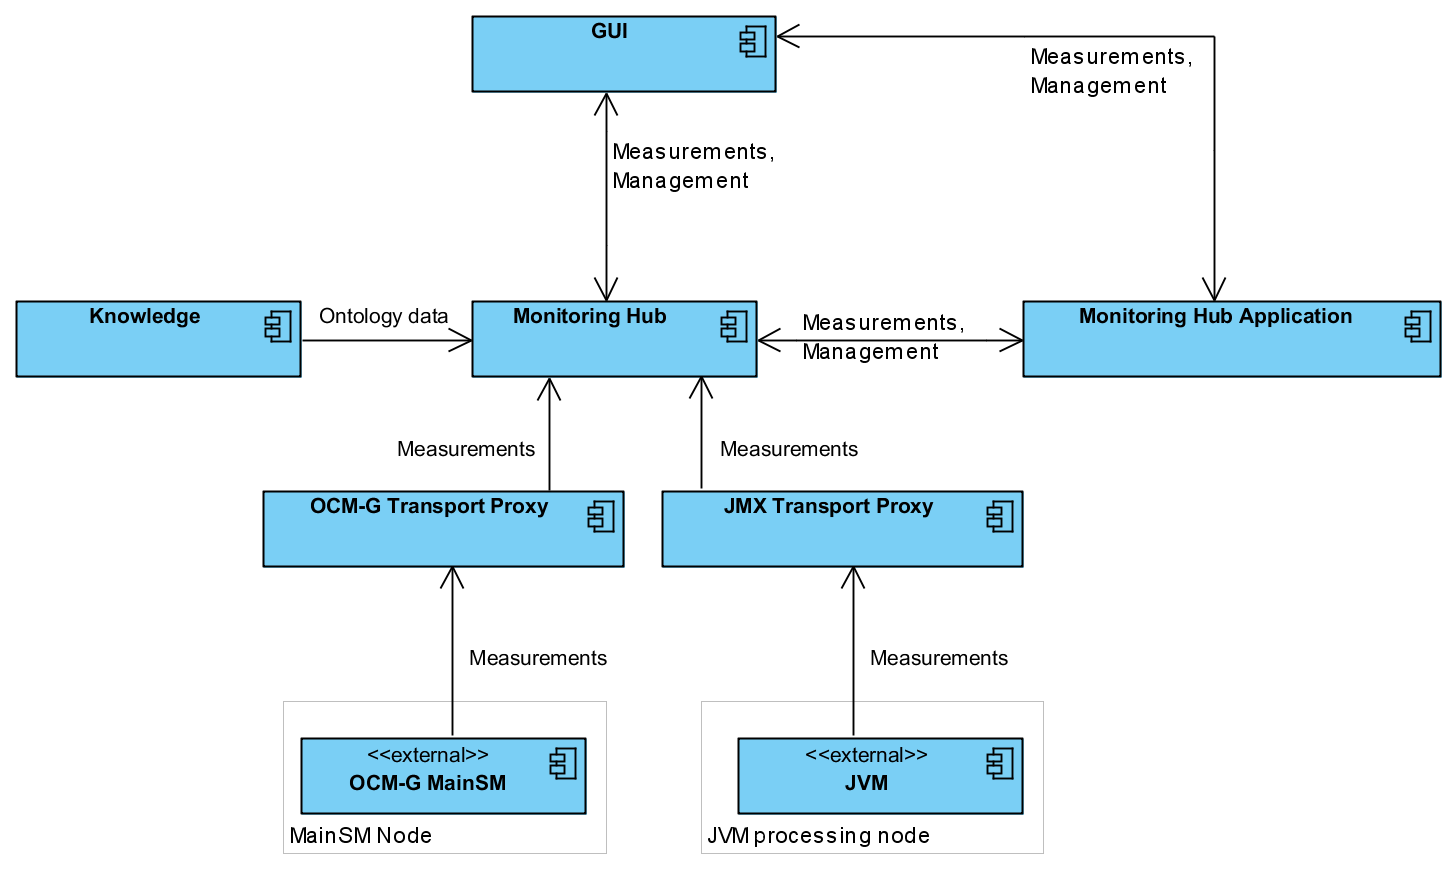
\includegraphics[width=1\textwidth]{arch_flows}
\caption{Overall system architecture}
\label{fig:arch_overall}
\end{figure}

At the design stage, several high level components have been introduced. All distinguished components, with relationships between them can be found in Figure~\ref{fig:decomposition_overall}. Each of these components should be interpreted as an independent one, which means that it is either a standalone application or a library, with API containing one or more interfaces. This API is then shared between the provider, which is a component that realizes the given interface and the consumer, a module that uses those functionalities to realize its own aims. The next subsection tries to list those components and describe them roughly.

\begin{figure}[ht]
\centering
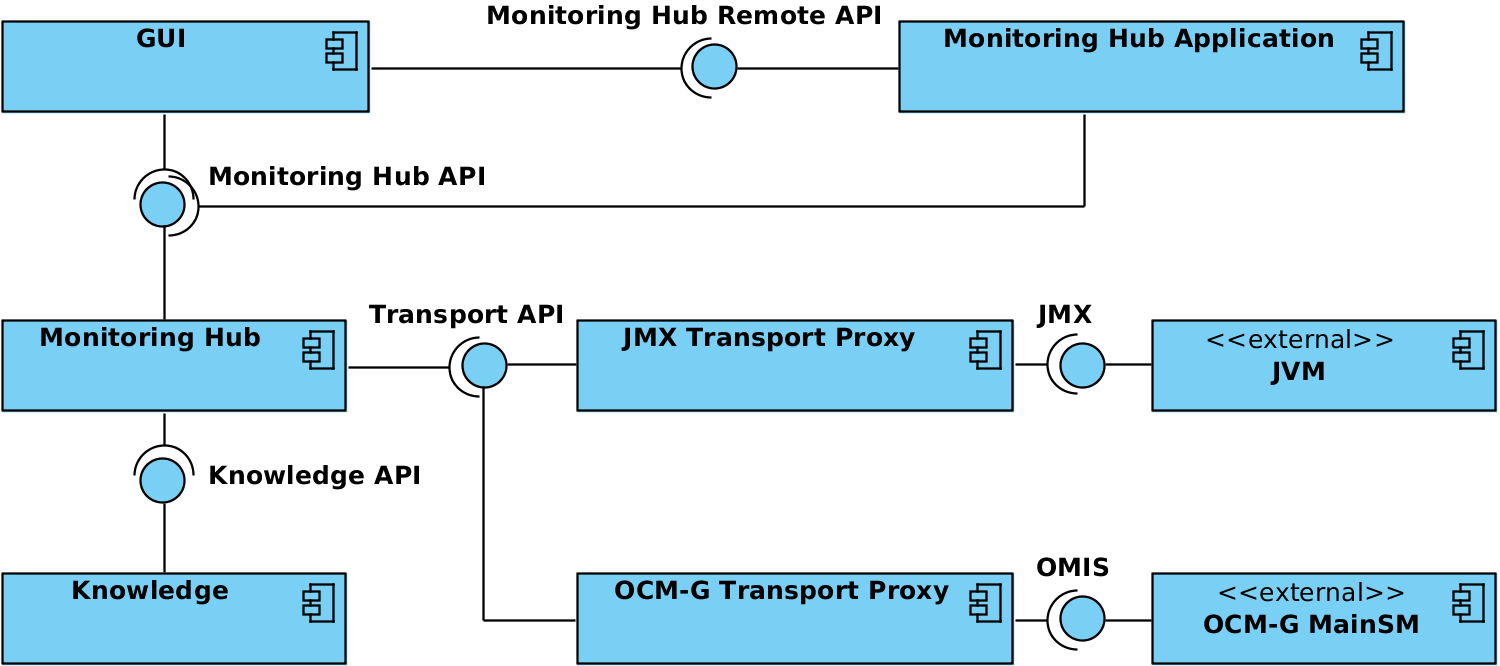
\includegraphics[width=1\textwidth]{arch_overall}
\caption{Overall system decomposition}
\label{fig:decomposition_overall}
\end{figure}

\subsection{Components overview}

As can be seen in Figure~\ref{fig:arch_overall}, the system has been decomposed into 8 high-level components. They are:

\begin{itemize}

\item {\bf GUI}~~~~~~~~~~~~~~~~~~~~~~~~~~~~~~~~~~~~~~~~~~~~~~~~~~~~~~~~\linebreak
Graphic User Interface is a standalone, desktop application, used directly by the user. It provides facilities that allow the management of the whole system. It does not perform any measurements or analysis. It only enables control over other components (direct or indirect) and visualizes the results of measurements.
The GUI application contains an embedded Monitoring Hub component, which allows the system to operate also in the smallest scale - a single measuring process with one or more measured processes attached directly. Additionally, it connects to the Monitoring Hub Application component, which allows using a remote Monitoring Hub.

\item {\bf Monitoring Hub}~~~~~~~~~~~~~~~~~~~~~~~~~~~~~~~~~~~~~~~~~~~~~~~~~~~~~~~~\linebreak
Monitoring hub is the most crucial component. Contains all the logic needed for a resource and a measurement management. It uses the Knowledge and Transport Proxies (one or more implementations) components to fulfill its duties. Only the JMX and the OCM-G transport proxies will be provided at this stage of a development, but the proposed architecture allows an easy addition of new proxies.
The Monitoring Hub does not work as a standalone application. Instead, it is in the form of a library (Java JAR) that other components will use. Additionally, the Monitoring Hub component is used by the GUI (in embedded mode) and the Monitoring Hub Application.

\item {\bf Monitoring Hub Application}~~~~~~~~~~~~~~~~~~~~~~~~~~~~~~~~~~~~~~~~~~~~~~~~~~~~~~~~\linebreak
Monitoring Hub Application will be a standalone, command line application (or a daemon if possible) that exposes services of the Monitoring Hub to other components with a remote access through the network (either LAN or WAN). It can accept remote connections from GUI components.
Its main responsibility is to allow the system to work in a distributed manner. Having a process that is separate, and independent from the GUI application, which continuously measures a work of the long-lasting jobs is crucial to allow the system to scale up.


\item {\bf Knowledge}~~~~~~~~~~~~~~~~~~~~~~~~~~~~~~~~~~~~~~~~~~~~~~~~~~~~~~~~\linebreak
The knowledge component realizes the semantics-based approach of the application. It provides ontology functionalities to the Monitoring Hub. It is responsible for initializing the ontology database and responses to all queries issued by the Monitoring Hub. These queries might be related to the relationships between resource types, resources or capabilities. This component is in a form of a library that is a dependency for the Monitoring Hub, and must be included in both the GUI and the Monitoring Hub Application distributions.

\item {\bf JMX Transport Proxy}~~~~~~~~~~~~~~~~~~~~~~~~~~~~~~~~~~~~~~~~~~~~~~~~~~~~~~~~\linebreak
A transport proxy component, which can communicate with JVM processes using the JMX protocol. Its main responsibilities include: establishing a connection with a JVM, mapping between a generic, knowledge-based resource or a capability value request into a Java component or a JMX query.

\item {\bf OCM-G Transport Proxy}~~~~~~~~~~~~~~~~~~~~~~~~~~~~~~~~~~~~~~~~~~~~~~~~~~~~~~~~\linebreak
A transport proxy component that communicates with an OCM-G MainSM monitor. Its responsibilities are similar to those of the JMX Transport Proxy: establish and maintain a connection to the MainSM, translate queries given in ontology terms to OMIS requests.

\end{itemize}

\subsection{Interfaces overview}

To decouple all the proposed components, the system will be using the following interfaces:

\begin{itemize}

\item {\bf Monitoring Hub API}~~~~~~~~~~~~~~~~~~~~~~~~~~~~~~~~~~~~~~~~~~~~~~~~~~~~~~~~\linebreak
It is an interface for the core system's logic. It describes methods that allow for management of every aspect of the system:  measurements, visualizations and resources. It is realized by the Monitoring Hub component and used by the GUI. 

\item {\bf Monitoring Hub Remote API}~~~~~~~~~~~~~~~~~~~~~~~~~~~~~~~~~~~~~~~~~~~~~~~~~~~~~~~~\linebreak
This interface is a derivative of the Monitoring Hub API. It contains the same set of functionalities, with addition of the operations specific to the remote access. This includes: registration of a remote listener, a remote interface wrapper for the Monitoring Hub allowing passing remote exceptions.

\item {\bf Transport API}~~~~~~~~~~~~~~~~~~~~~~~~~~~~~~~~~~~~~~~~~~~~~~~~~~~~~~~~\linebreak
The Transport API is a common interface for a communication with data access services. Currently it is implemented by the JMX and the OCM-G Transport Proxy components. To add support for other data sources in the future, it is necessary to implement this interface.

\item {\bf Knowledge API} ~~~~~~~~~~~~~~~~~~~~~~~~~~~~~~~~~~~~~~~~~~~~~~~~~~~~~~~~\linebreak
Interface describing operations related to the ontology maintenance and usage. This interface is realized by the Knowledge component and used by Monitoring Hub. 

\end{itemize}

\subsection{Most important data flows}

Figure~\ref{fig:comm_add_resource} contains the communication diagram covering the add a new resource action. This action is initialized by the user actor. User starts a flow by performing an action (like button click or wizard - not covered here) on the GUI component. In a response to this event, the GUI sends a request to the Monitoring Hub, asking to register the new resource, using parameters provided by the user. In the subsequent step, the Monitoring Hub first looks up in its dictionary of all registered transport proxies, for the one that can communicate with a resource specified by the user. After finding a valid transport proxy, it passes the registration request to it. In this case, the JMX Transport Proxy tries to initialize a connection to the JVM using a URL provided by the user in the first step. After a successful connection, the JmxTransportProxy creates and initializes a Resource object. This process includes gathering basic attributes, describing the object as well as setting all meta data that the proxy will need to operate with a given resource, in the future. After finishing this step, a fully initialized resource is being returned to the Monitoring Hub. Knowing that the transport proxy has been properly attached to the newly registered resource, the Monitoring Hub notifies about a new resource all listeners, in this case the GUI component. After issuing this notification, it will try to discover all children of this resource. To do it, first it must obtain URLs of child types, so it sends a request to the Knowledge component. Having the types of the child resources, the Monitoring Hub requests the transport proxy to discover the children of an already registered resource and of the given types. Again, in this case the JMX transport proxy will translate a discovery request into JMX queries, to discover the child resources. Discovered children are then returned to the Monitoring Hub as resource objects. All these objects are registered by the Monitoring Hub and a notification is being issued to the listeners.

\begin{figure}[ht]
\centering
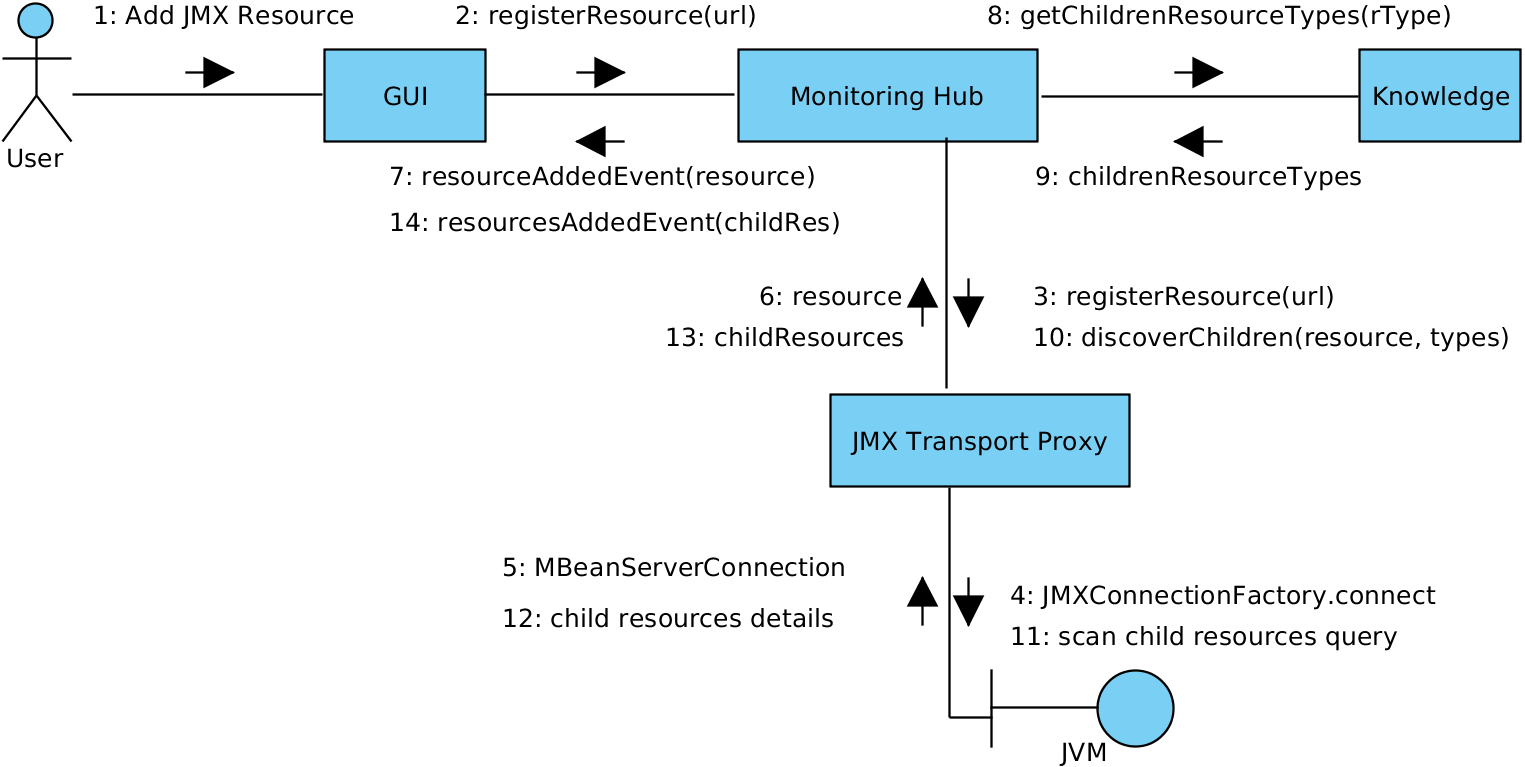
\includegraphics[width=0.9\textwidth]{comm_add_resource}
\caption{Communication diagram - adding of new resource}
\label{fig:comm_add_resource}
\end{figure}

The addition of a new measurement is a bit simpler than the registration of new resources. The message exchange needed to achieve it can be found in Figure~\ref{fig:comm_add_measurement}. In this case, similarly as above, the action is initialized by user. He or she chooses a resource to add a relevant measurement, and clicks an appropriate button. In reaction to this event, the GUI requests the Monitoring Hub to get all possible capabilities that can be measured for the type of a resource selected by user. The Monitoring Hub passes this request to the Knowledge component. Then, a result goes back to the GUI, which can render an appropriate user interface item that will allow the user to select which capability to measure. After having selected a capability by user, GUI issues a request to add the new measurement to the Monitoring Hub. The request contains both the resource identifier and an ontology URL of the capability. Monitoring Hub then verifies, whether the selected capability can be measured with the selected resource. Such a validation is needed, because in certain circumstances it might be unfeasible, e.g. not every transport proxy is able to measure a given capability of a resource. To check this, Monitoring Hub sends a verification request to the transport proxy (the JMX Transport Proxy in the example from Figure~\ref{fig:comm_add_measurement}). After a successful verification, the Monitoring Hub initializes a scheduled job that will poll for the capability values - the measurement is successfully created and started.

\begin{figure}[ht]
\centering
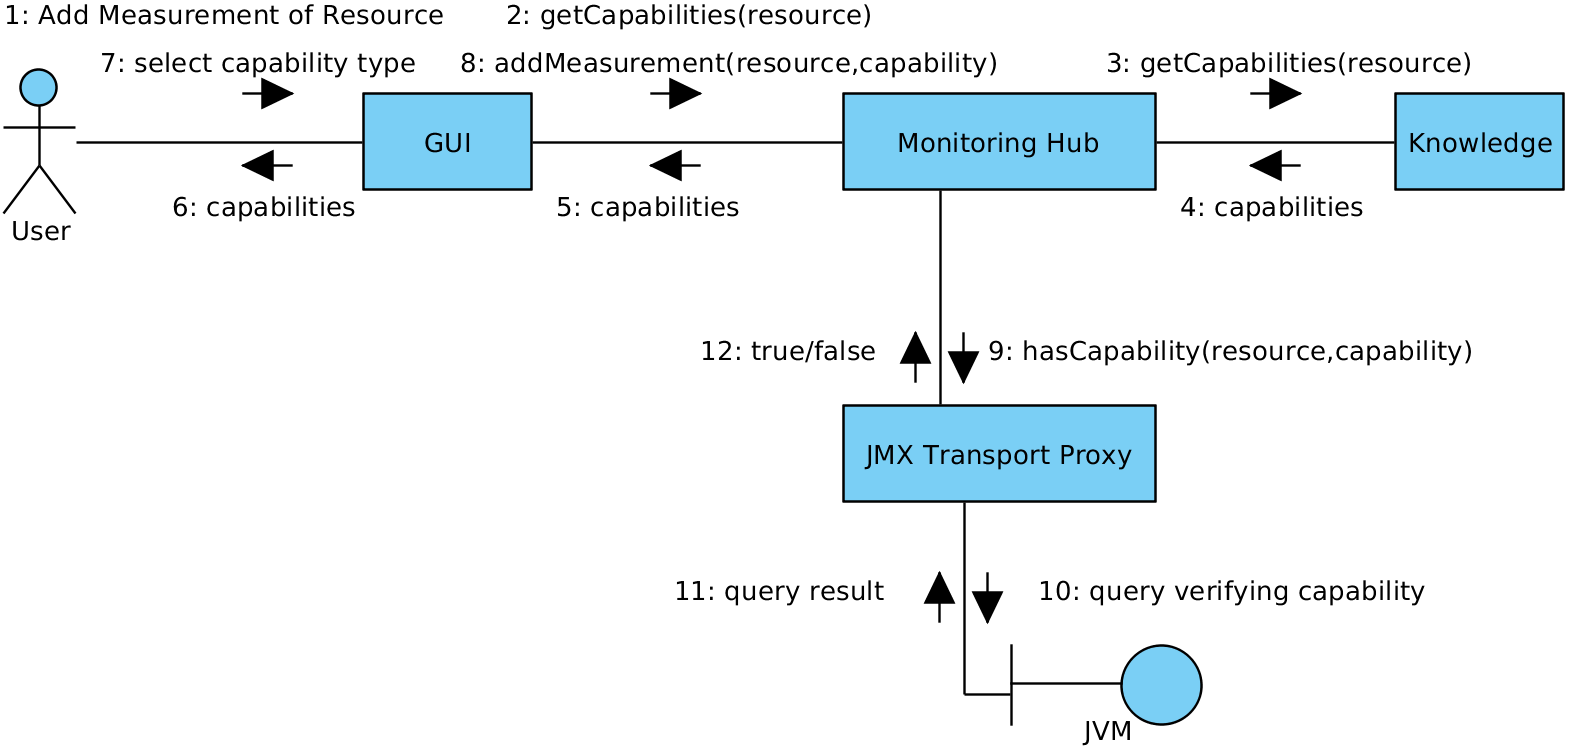
\includegraphics[width=0.9\textwidth]{comm_add_measurement}
\caption{Communication diagram - adding of new measurement}
\label{fig:comm_add_measurement}
\end{figure}

Publishing a new capability value is definitely the most frequently used data flow in the whole system. Figure~\ref{fig:comm_new_cap_value} depicts this process. In contrast to the previous communication diagrams, in this case the Monitoring Hub component is the initiator of this operation. The logic of this component manages scheduled jobs responsible for polling a new capability value, and then pushing it to the listeners, the previously registered GUI components. In the first step, Monitoring Hub calls an appropriate (the one associated with resource in question) transport proxy, which is JMX Transport Proxy in this case. JMX Transport Proxy maps a generic \texttt{getCapabilityValue} request into a specific JMX query, sends the query to the monitored JVM and returns a result to the Hub. The Monitoring Hub uses this result to issue a notification dispatched through all the registered listeners. The GUI component, receives an event and updates a visualization graph, which is being watched by user.

\begin{figure}[ht]
\centering
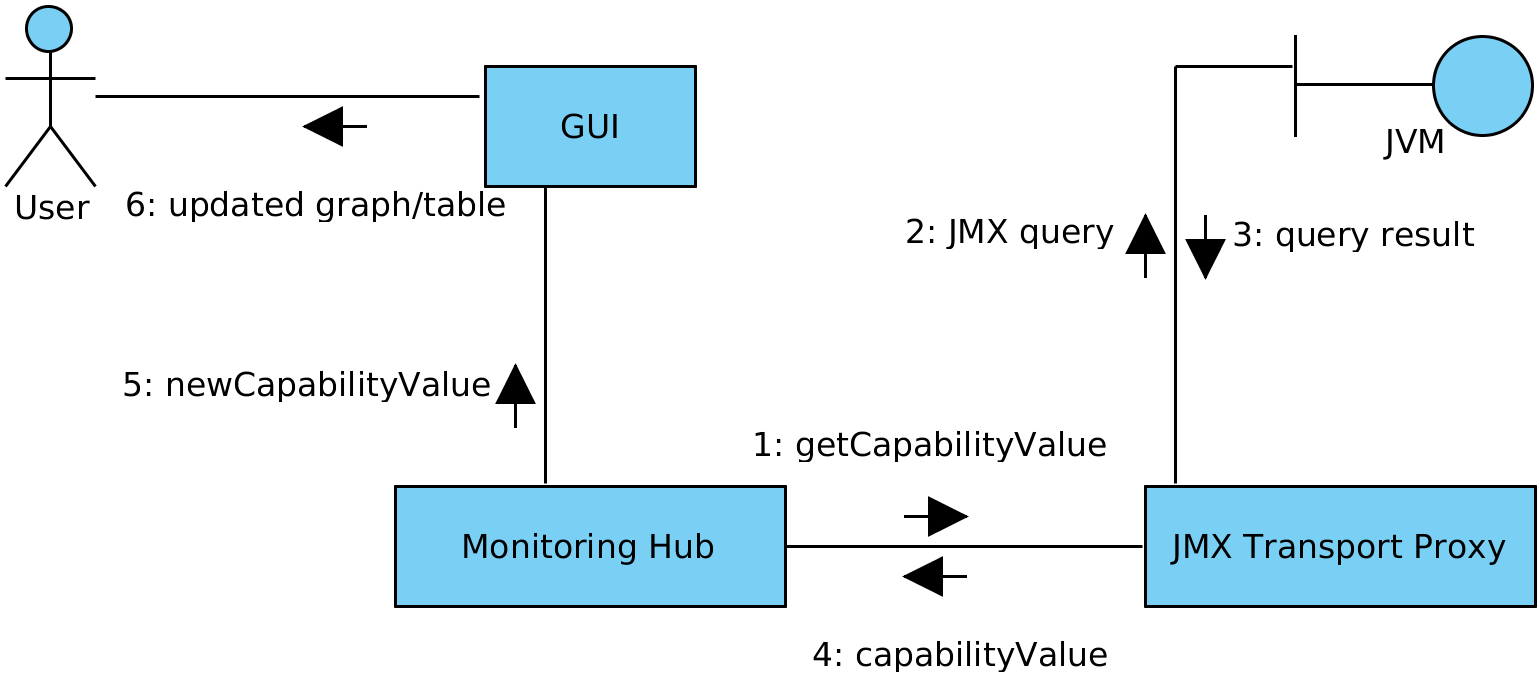
\includegraphics[width=0.7\textwidth]{comm_new_cap_value}
\caption{Communication diagram - new capability value}
\label{fig:comm_new_cap_value}
\end{figure}


\subsection{Communication protocol}
\label{subsec:arch_comm_protocol}

The Communication protocol between components must allow both types of interactions: local and remote. By a local interaction I mean the one, where all components constitute a single process and share the same memory space. The system must use a remote interaction, when one or more components works as a separate process to other, which enforces the usage of network stack for messages exchange. To make it possible, all communications will be performed using predefined, plain interfaces, which are not aware of the underlying communication type. Such an approach decouples a communication schema from a networking protocol being employed.

As a general rule for all message exchanges between components, transfer object (also known as value object) design pattern will be used~\cite{0131422464}. This allows for decoupling the content of message of any complexity from the serialization mechanisms used. The following tables list all transfer objects used in the system. Additionally the reader may find a short description of each object;s rationale behind each member. 

% Add vertical spacing
\renewcommand*\arraystretch{1.2}

\begin{table}[ht] % ======================== CapabilityValue =====================================
\begin{tabular}{| m{1,5cm} | m{3,2cm} | m{8,5cm} |}
\hline 
\cellcolor[gray]{0.9} Field Type & \cellcolor[gray]{0.9} Field Name & \cellcolor[gray]{0.9} Details \\
\hline 
Number & \texttt{numberValue} & Numeric value of capability (optional, must be set if \texttt{ValueType} is number) \\
Number[] & \texttt{arrayValue} & Vector value of capability (optional, must be set if \texttt{ValueType} is vector) \\
ValueType & \texttt{valueType} & Type of capability value - either numeric or vector\\
Date & \texttt{gatherTimestamp} & Timestamp in UTF, when capability value have been gathered \\
String & \texttt{metricsId} & Id of measurement to which this capability value belongs \\
\hline 
\end{tabular}
\caption{List of members of \texttt{CapabilityValue} Transfer Object}
\label{tab:TO_CapValue}
\end{table} % ======================== CapabilityValue =====================================

Table~\ref{tab:TO_CapValue} contains a list of members of the \texttt{CapabilityValue} transfer object. This object is used to notify listeners (GUI) about new capability values, and acts mostly as a container for value, with additional metadata. The most significant additional property that each \texttt{CapabilityValue} has is the \texttt{gatherTimestamp} which points to the exact moment of time, when this capability value has been gathered. Using this property, the system can use \texttt{CapabilityValue} transfer objects, without worrying about the implication of processing time on a measurements presentation.

Members of the \texttt{MeasurementDefinition} message can be found in Table~\ref{tab:TO_MeasurementDef}. This object is used by the GUI component to define a measurement that should be created.

\begin{table}[ht] % ======================== MeasurementDefinition =====================================
\begin{tabular}{| m{1,5cm} | m{3,2cm} | m{8,5cm} |}
\hline 
\cellcolor[gray]{0.9} Field Type & \cellcolor[gray]{0.9} Field Name & \cellcolor[gray]{0.9} Details \\
\hline 
String & \texttt{resourceUri} & URI of resource that is covered by this measurement \\
String & \texttt{capabilityUri} & URI of capability that is covered by this measurement \\
long & \texttt{updateInterval} & Interval in milliseconds defining how frequently the value of measurement will be polled \\
String & \texttt{id} & Identifier of this measurement \\ 
\hline 
\end{tabular}
\caption{List of members of \texttt{MeasurementDefinition} transfer object}
\label{tab:TO_MeasurementDef}
\end{table} % ======================== MeasurementDefinition =====================================

The following tables:~\ref{tab:TO_Resource} and \ref{tab:TO_ResourceEvent} contain a definition of transfer objects needed for the resource management. Resource transfer object contains a complete description of resource managed by the system, additionally the Monitoring Hub uses \texttt{ResourceEvent} to notify all listeners (GUI mostly) about resource's life cycle events. 

\begin{table}[ht] % ======================== Resource =====================================
\begin{tabular}{| m{1,5cm} | m{3,2cm} | m{8,5cm} | }
\hline 
\cellcolor[gray]{0.9} Field Type & \cellcolor[gray]{0.9} Field Name & \cellcolor[gray]{0.9} Details \\
\hline
String & \texttt{typeUri} & URI of resource\rq{}s type according to currently used ontology \\
String & \texttt{uri} & URI of resource in current resources tree hierarchy \\
Map & \texttt{properties} & Static properties of resource (e.g. OS version) \\
\hline 
\end{tabular}
\caption{List of members of \texttt{Resource} transfer object}
\label{tab:TO_Resource}
\end{table} % ======================== Resource =====================================

\begin{table}[ht] % ======================== ResourceEvent =====================================
\begin{tabular}{| m{1,5cm} | m{3,2cm} | m{8,5cm} | }
\hline 
\cellcolor[gray]{0.9} Field Type & \cellcolor[gray]{0.9} Field Name & \cellcolor[gray]{0.9} Details \\
\hline
Type & \texttt{eventType} & Enumeration that defines whether resources in this event have been added or removed \\
List & \texttt{resources} & Collections of resources covered by this event \\
\hline 
\end{tabular}
\caption{List of members of \texttt{ResourceEvent} transfer object}
\label{tab:TO_ResourceEvent}
\end{table} % ======================== ResourceEvent =====================================
% Remove vertical spacing
\renewcommand*\arraystretch{1}

